\section{Results}\label{sec:results}
\begin{framed}
6. Implement and test a part of your system using the ZYBO platform including at least one IP core written and verified with the HLS tool.
\end{framed}

This sections shows the results in performance and utilization of all the designs we have been through, that is a high-level synthesis of the two IP cores (GenerationGenerator and Simulator) and the user application, that was implemented and deployed to the ZYBO board. Overall, our results show that simple fixed-point arithmetic can be accelerated in an hardware FPGA at relative low cost, however more complicated floating point computations are better done in software, as the number of required DSP's and lookup tables rapidly increase in such cases.

\subsection{HLS of the GenerationGenerator core}

\begin{figure}[h]
	\centering
	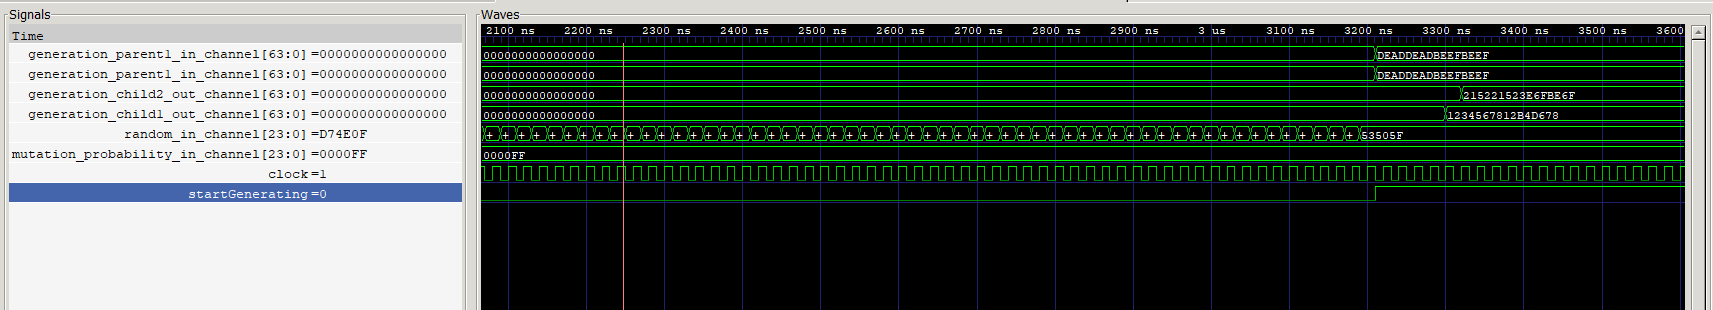
\includegraphics[width=1.0\linewidth]{../diagrams/GenerationGeneratorSim.png}
	\caption{A trace diagram that shows all bidirectional signals of the module.}
	\label{fig:generationgeneratortrace}
\end{figure}

\subsection{HLS of the Simulator core}
\subsection{User application and performance}




